\documentclass[t, pdftex]{beamer}  
%Use Cockrell School Theme.  Optional department name.  Must %ecape, i.e. use 
%backslash, to preserve spaces.  The default is ``Cockrell School of Engineering''
\usetheme[]{cockrell}                 
%\usetheme[dept=Aerospace\ Engineering\ and\ Engineering\ Mechanics]{cockrell}                 
%\usetheme[dept=Biomedical\ Engineering]{cockrell}                 
%\usetheme[dept=Chemical\ Engineering]{cockrell}                 
%\usetheme[dept=Civil,\ Architectural\ and\ Environmental\ Engineering]{cockrell}                 
%\usetheme[dept=Electrical\ and\ Computer\ Engineering]{cockrell}                 
%\usetheme[dept=Mechanical\ Engineering]{cockrell}                 
%\usetheme[dept=Materials\ Science\ and\ Engineering]{cockrell}                 
%\usetheme[dept=Petroleum\ and\ Geosystems\ Engineering]{cockrell}                 

% Add preamble packages here
%\usepackage{etex}
%\usepackage[bigfiles]{media9}
%\graphicspath{{./figs/}}

%Enable cancelto in math
\usepackage{cancel}
\usepackage{amsmath}
\usepackage[fleqn]{mathtools}
\usepackage{amssymb}
\usepackage{amsthm}
\usepackage{enumitem}
\renewcommand{\CancelColor}{\color{utorange}}

%Add bibliography file location for citiation
\bibliography{}


\title{A Summary of Research}
\subtitle{Disaster Repair}
\author{Brian French}
\institute{Department of Industrial Engineering}
\date{\today}


\begin{document}

%Creates title frame from title, subtitle, author, institute, and date above
\titleframe 
%Supports table of contents
\frame{\frametitle{Outline}\tableofcontents}

%Section commands will define what's shown in TOC
\section{Posing the Problem}

%First frame
\begin{frame}
    \frametitle{Reasons to Address}

    \begin{itemize}
        %Support for external hyperlinks as shown
        \item Hurricanes increasing in frequency and intensity
        \item Previous work is overly reductive 
        \item Almost no work dealing with multiple infrastructure layers
        \item Roads and power grids both have interesting properties of their own
    \end{itemize}
\end{frame}

\begin{frame}
    \frametitle{Method of Addressing}

    \begin{itemize}
        \item Treat as a two actor game
        \item Find both transit and electrical ideal repair schedules
        \item Find ideal transit repair conditional on electrical getting whatever they want
        \item Find ideal electrical repair conditional on transit repair getting whatever they want
        \item do some sort of comparison or iteration to find a consensus solution?
    \end{itemize}
\end{frame}
\section{Power Model Example}
\begin{frame}
	\frametitle{Sets and Indices}
	\begin{itemize}
		\item $N$ is the set of nodes, indexed by $i$
		\item $E$ is the set of power lines, indexed by $e$
		\item $R$ is the set of road segments
		\item $T$ is the planning horizon, indexed by $t$
		\item $O(i)$ is the set of lines with origin $i$
		\item $D(i)$ is the set of lines with destination $i$
		\item $o(e)$ is the origin node of line $e$
		\item $d(e)$ is the destination node of line $e$
	\end{itemize}

\end{frame}
\begin{frame}
\frametitle{Parameters and Data}
\begin{itemize}
	\item $\underline{L_e}$ and $\overline{L_e}$ is the capacity lower and upper bounds for the power line $e$
	\item $\Delta_{i}$ is the time to repair node $i$ and $\delta_{e}$ is the time to repair line $e$
	\item $C_{SP(i)}$ is the length of the shortest path to node $i$ from the central depot
	\item $K$ is a coefficient of "broken-ness" representing the average slowdown from debris on the road and minor flooding
	\item $D_i$ is the power demand at location $i$ in the pre-disaster steady state
	\item $P_k$ is the maximum power generation for generator $k$
	\item $B_e$ is the line susceptance (imaginary part of admittance, also inverse of resistance) for power line $e$
	\item $I_e, I_i$ is the initial condition of line $e$ and node $i$, respectively.
\end{itemize}
\end{frame}
\begin{frame}
\frametitle{The Model}
Objective:
$$ \min \sum_{i \in N} \sum_{t \in T} (1-W_i^t)D_i $$
Subject to:
	\begin{enumerate}[label=(\arabic*), leftmargin=*, itemsep=0.4ex, before={\everymath{\displaystyle}}]
	
	\item $ X_e^t = B_e * (\theta_{o(e)}^t - \theta_{d(e)}^t), \hspace{5pt} \forall t \in T, \hspace{4pt} \forall e \in E$
	\item $ G_i^t - \sum_{l \in O(i)} X_l^t + \sum_{l \in D(i)} X_l^t = D_i, \hspace{4pt} \forall t \in T, \hspace{4pt} \forall i \in N$
	\item $G_k^t \leq P_{k} V_{k}^t, \hspace{4pt} \forall t \in T, \hspace{4pt} \forall k \in N$
	\item $\underline{L_e}W_{e}^t \leq X_{e}^t \leq \overline{L_e}W_{e}^t, \hspace{4pt} \forall t \in T, \hspace{4pt} \forall e \in E$
	\item $\underline{L_e}V_{o(e)}^t \leq X_{e}^t \leq \overline{L_e}V_{o(e)}^t, \hspace{4pt} \forall t \in T, \hspace{4pt} \forall e \in E$
	\item $\underline{L_e}V_{d(e)}^t \leq X_{e}^t \leq \overline{L_e}V_{d(e)}^t, \hspace{4pt} \forall t \in T, \hspace{4pt} \forall e \in E$
	\end{enumerate}
These 6 constraints define the mathematical rules for operation of a damaged DC-approximated power grid.
\end{frame}
\begin{frame}
\frametitle{Model Continued}
	\begin{enumerate}[label=(\arabic*), leftmargin=*, itemsep=0.4ex, before={\everymath{\displaystyle}}]
	\item $MST^t = \sum_{i \in N} \sum_{j \in N} SP_{ij}*Z_{ij}^{t} C_{speed}\hspace{4pt} \forall t \in T $
	\item $\sum_{i \in N} \sum_{j \in N} Z_{ij}^{t} >= \sum_{i \in N} F_i^t + \sum_{e \in E} S_e^t - \sum_{i \in N} F_i^t \sum_{O(i)} S_e^t - \sum_{i \in N} F_i^t \sum_{D(i)} S_e^t \hspace{4pt} \forall t \in T$
	\item $\sum_{i,j \in S} Z_{ij}^t <= |s|-1 \hspace{4pt} S\subset N$
	\item $ \sum_{j \in N} Z_{ij}^t \geq F_i^t \hspace{4pt} \forall t \in T\hspace{4pt} \forall i \in N $
	\item $ \sum_{e \in E} \delta_{e}S_e^t + \sum_{i \in N}\Delta_{i}F_i^t + MST_t <=8$
\end{enumerate}

\end{frame}
\begin{frame}
\frametitle{Model Continued}
	\begin{enumerate}[label=(\arabic*), leftmargin=*, itemsep=0.4ex, before={\everymath{\displaystyle}}]
\item $V_i^t \leq \sum_{t'=0}^{t-1} F_i^{t'}+I_i, \hspace{4pt} \forall i \in N$ 
\item $W_{e}^t \leq \sum_{t'=0}^{t-1} S_{e}^{t'}+I_e, \hspace{4pt} \forall e \in E $
\end{enumerate}
These first 4 constraints outline the rules to construct a spanning tree that is minimal in some cases and "short enough" in others, the two constraints on the slide after govern functionality of a node based on its repair status.
\end{frame}

\begin{frame}
\frametitle{Grid Layout}
\begin{figure}
\caption{IEEE Bus30(green) with roads(red) }
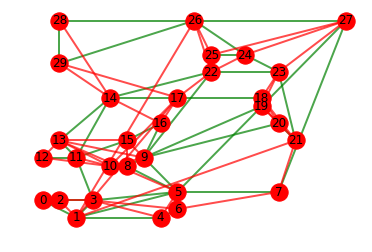
\includegraphics[scale=.5]{GridLayout.png}
\end{figure}
\end{frame}
\section{Current Work}
\begin{frame}
\frametitle{Current State}
\begin{itemize}
	\item -Road repair model based on routing
	\item -DC Power grid repair model approximating routing with MST
	\item -DC Power grid repair conditional on optimal road repair
\end{itemize}
\end{frame}
\begin{frame}
\frametitle{Modeling Next Steps}
\begin{itemize}
	\item -Inclusion of multiple levels of damage to roads (debris/flood/severe blockage)
	\item -Road repair conditional on optimal power grid repair
	\item -Development of iteration framework to balance the two competing objectives
	\item -Inventory prepositioning model
\end{itemize}
\end{frame}
\end{document}
